%%%%%%%%%%%%%%%%%%%%%%%%%%%%%%%%%%%%%%%%%%%%%%
%                insertmeeting
% 1) Title (something creative & funny?)
% 2) Date (MM/DD/YYYY)
% 3) Location (ex. Hagerty High School)
% 4) People/Committees Present 
% 5) Picture 
% 6) Start Time & Stop Time (ex. 12:30AM to 4:30PM)
%%%%%%%%%%%%%%%%%%%%%%%%%%%%%%%%%%%%%%%%%%%%%%
\insertmeeting 
	{Reevaluation Revolution} 
	{01/09/22} 
	{Hagerty High School}
	{Jensen}
	{Images/RobotPics/robot.jpg}
	{2:30 - 4:30}
	
\hhscommittee{Hardware}
\noindent\hfil\rule{\textwidth}{.4pt}\hfil
\subsubsection*{Goals}
\begin{itemize}
    \item Re evaluate design for intake
    \item Come up with a way to prevent launching while out taking
 

\end{itemize} 

\noindent\hfil\rule{\textwidth}{.4pt}\hfil

\subsubsection*{Accomplishments}
Our original design idea for our out-take system, which is integrated with the intake, was to have a trap door on the top which would open, releasing the game element after the intake flips over into scoring position. Although this design is good for preventing launching, a rule which has affected some other teams in our league while out-taking, it will not be able to score in the middle goal and will require the arm to be higher to score in the top goal. To illustrate this problem, we created a quick sketch of what would happen with the current design (Figure \ref{fig:010922_1}). As shown in the image, dropping the block out of the trap door at the top (pictured on the bottom in the sketch) doesn’t allow enough clearance to back out of the hub without descoring the block. Because our intake would have to be entirely above the block when dropping it, it would require us to have 2 inches between the desired level of the shipping hub and the lowest point of the intake/out-take, leaving us with only around a 4 inch zone to put our intake in. Even if the intake is small enough to fit in this zone, ensuring that it is at the exact height it needs to be at will be very difficult. This issue will only be amplified if the sipping hub tips. Because of this, using the trap door idea isn’t feasible.
While coming up with new ideas, we had the idea to out take the same way we intake, but in reverse. Instead of spinning the spinner to suck the block in, we would spin it in the opposite direction to push the block out. Although this idea would work better than the trap door, it still leaves us open to the risk of a launching penalty, which, considering the speed of our intake, seems pretty likely. To fix this, we plan on having our software committee slow down the sweeper when going in reverse, to hopefully push the block out gently. Luckily, we didn’t have to make any significant changes in CAD because we had yet to design the trap door and our new solution uses pre-existing  features of the robot.

 

\begin{figure}[htp]
\centering
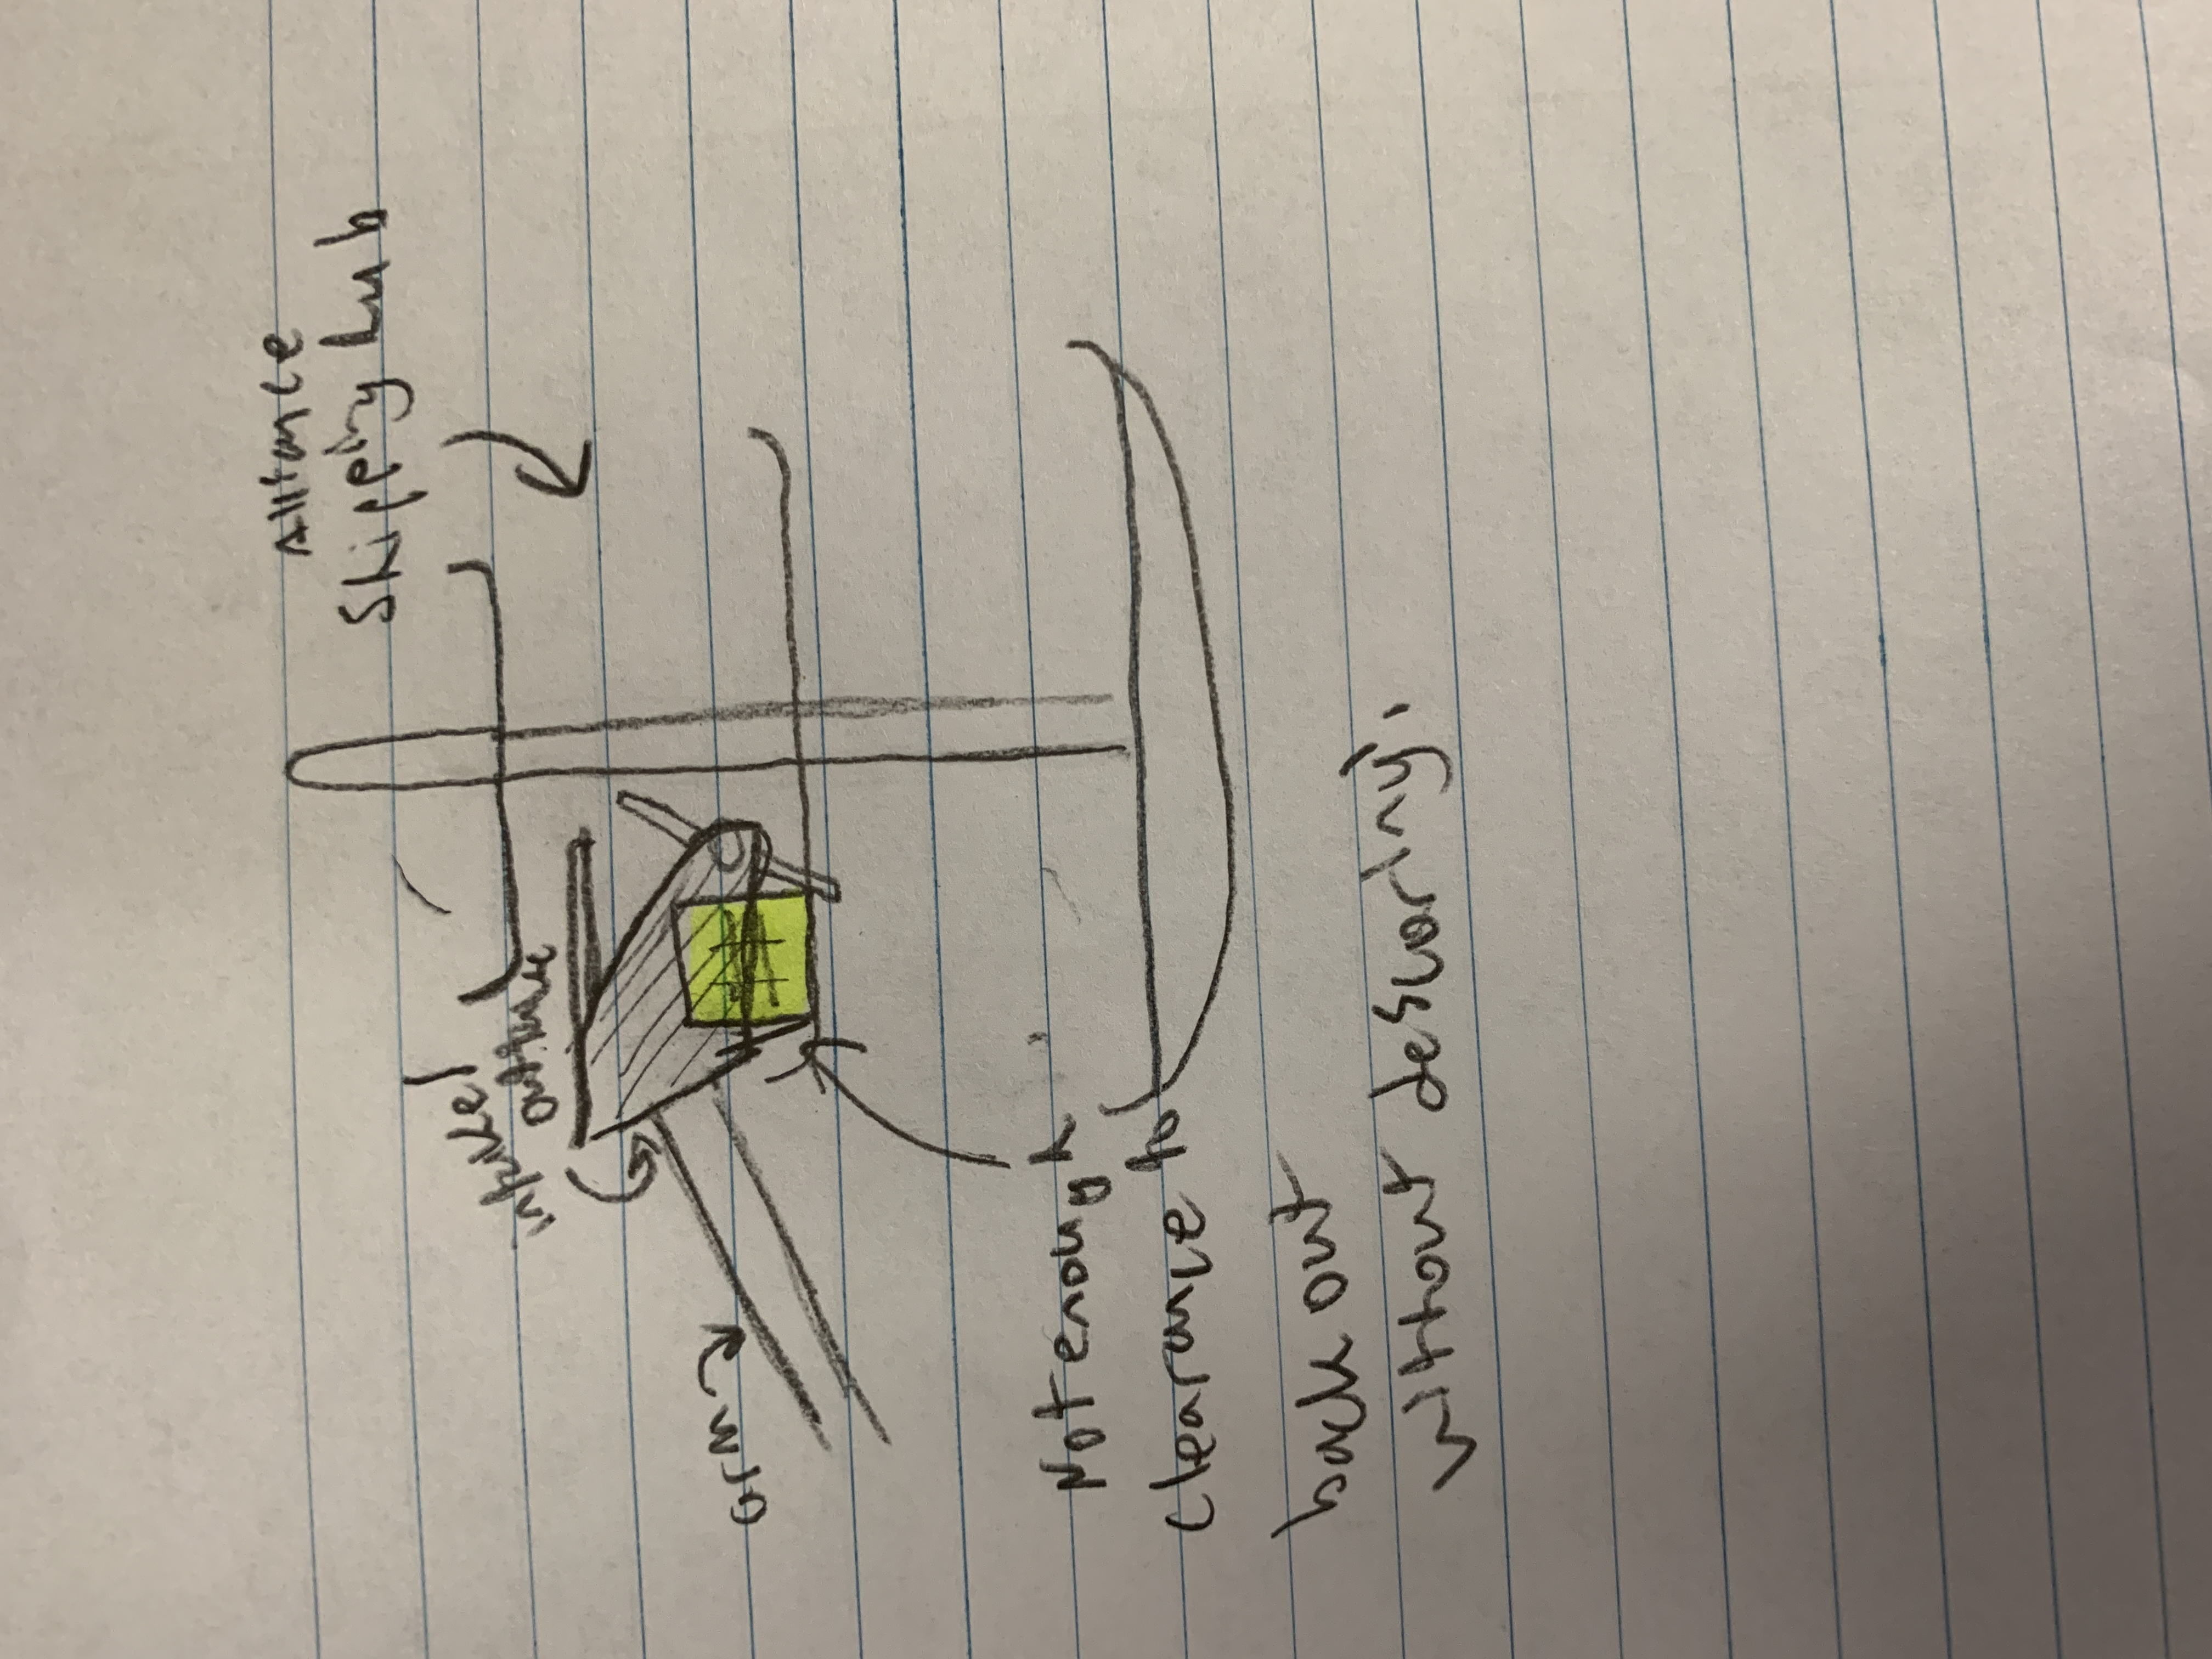
\includegraphics[width=0.95\textwidth, angle=0]{Meetings/January/01-09-22/IMG_3223 - Nathan Forrer.JPG}
\caption{Our current design sketched out}
\label{fig:010922_1}
\end{figure}

\whatsnext{
\begin{itemize}
    \item Laser cut and 3D print parts for sweeper intake
    \item Build and test sweeper intake

\end{itemize} 
}

